\section{Bios}
\label{sec:bios}

\parbox{6.5in}{
\begin{wrapfigure}{r}{3.6in - .75\columnsep} %{3.8in}{0.45\textwidth}
  % \centering
    \vspace{-\intextsep}
    \hspace*{-.35\columnsep}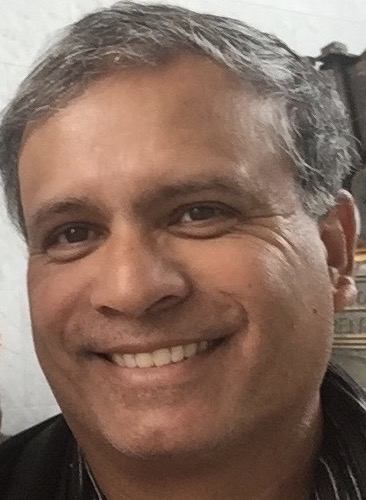
\includegraphics[scale=0.4]{fig/KRajan.jpg}
\end{wrapfigure}
\textbf{Kanna Rajan} is a Fellow at SIFT LLC and holds a visiting
faculty appointment at \univ in autonomous systems. At \nas his
software was responsible for the command/control of the 1999 New
Millennium Deep Space 1, 65 Million miles from Earth and the 2003 Mars
Exploration Rovers mission on the Red Planet. In 2005 he moved to \mba
to build the only AI group in marine robotics and to focus on using
AI-based machine intelligence for marine robotics and biological
oceanography. His publications have been in highly ranked
peer-reviewed publications while his field work includes scientific
oceanographic cruises in the Pacific and the Atlantic.\\

\textbf{email: }\emph{Kanna.Rajan@fe.up.pt}\\
\textbf{Web: }\url{https://kanna.rajan.systems}
}

\vspace{20mm}

\parbox{6.5in}{
\begin{wrapfigure}{r}{3.6in - .75\columnsep} %{3.8in}{0.45\textwidth}
  % \centering
    \vspace{-\intextsep}
    \hspace*{-.35\columnsep}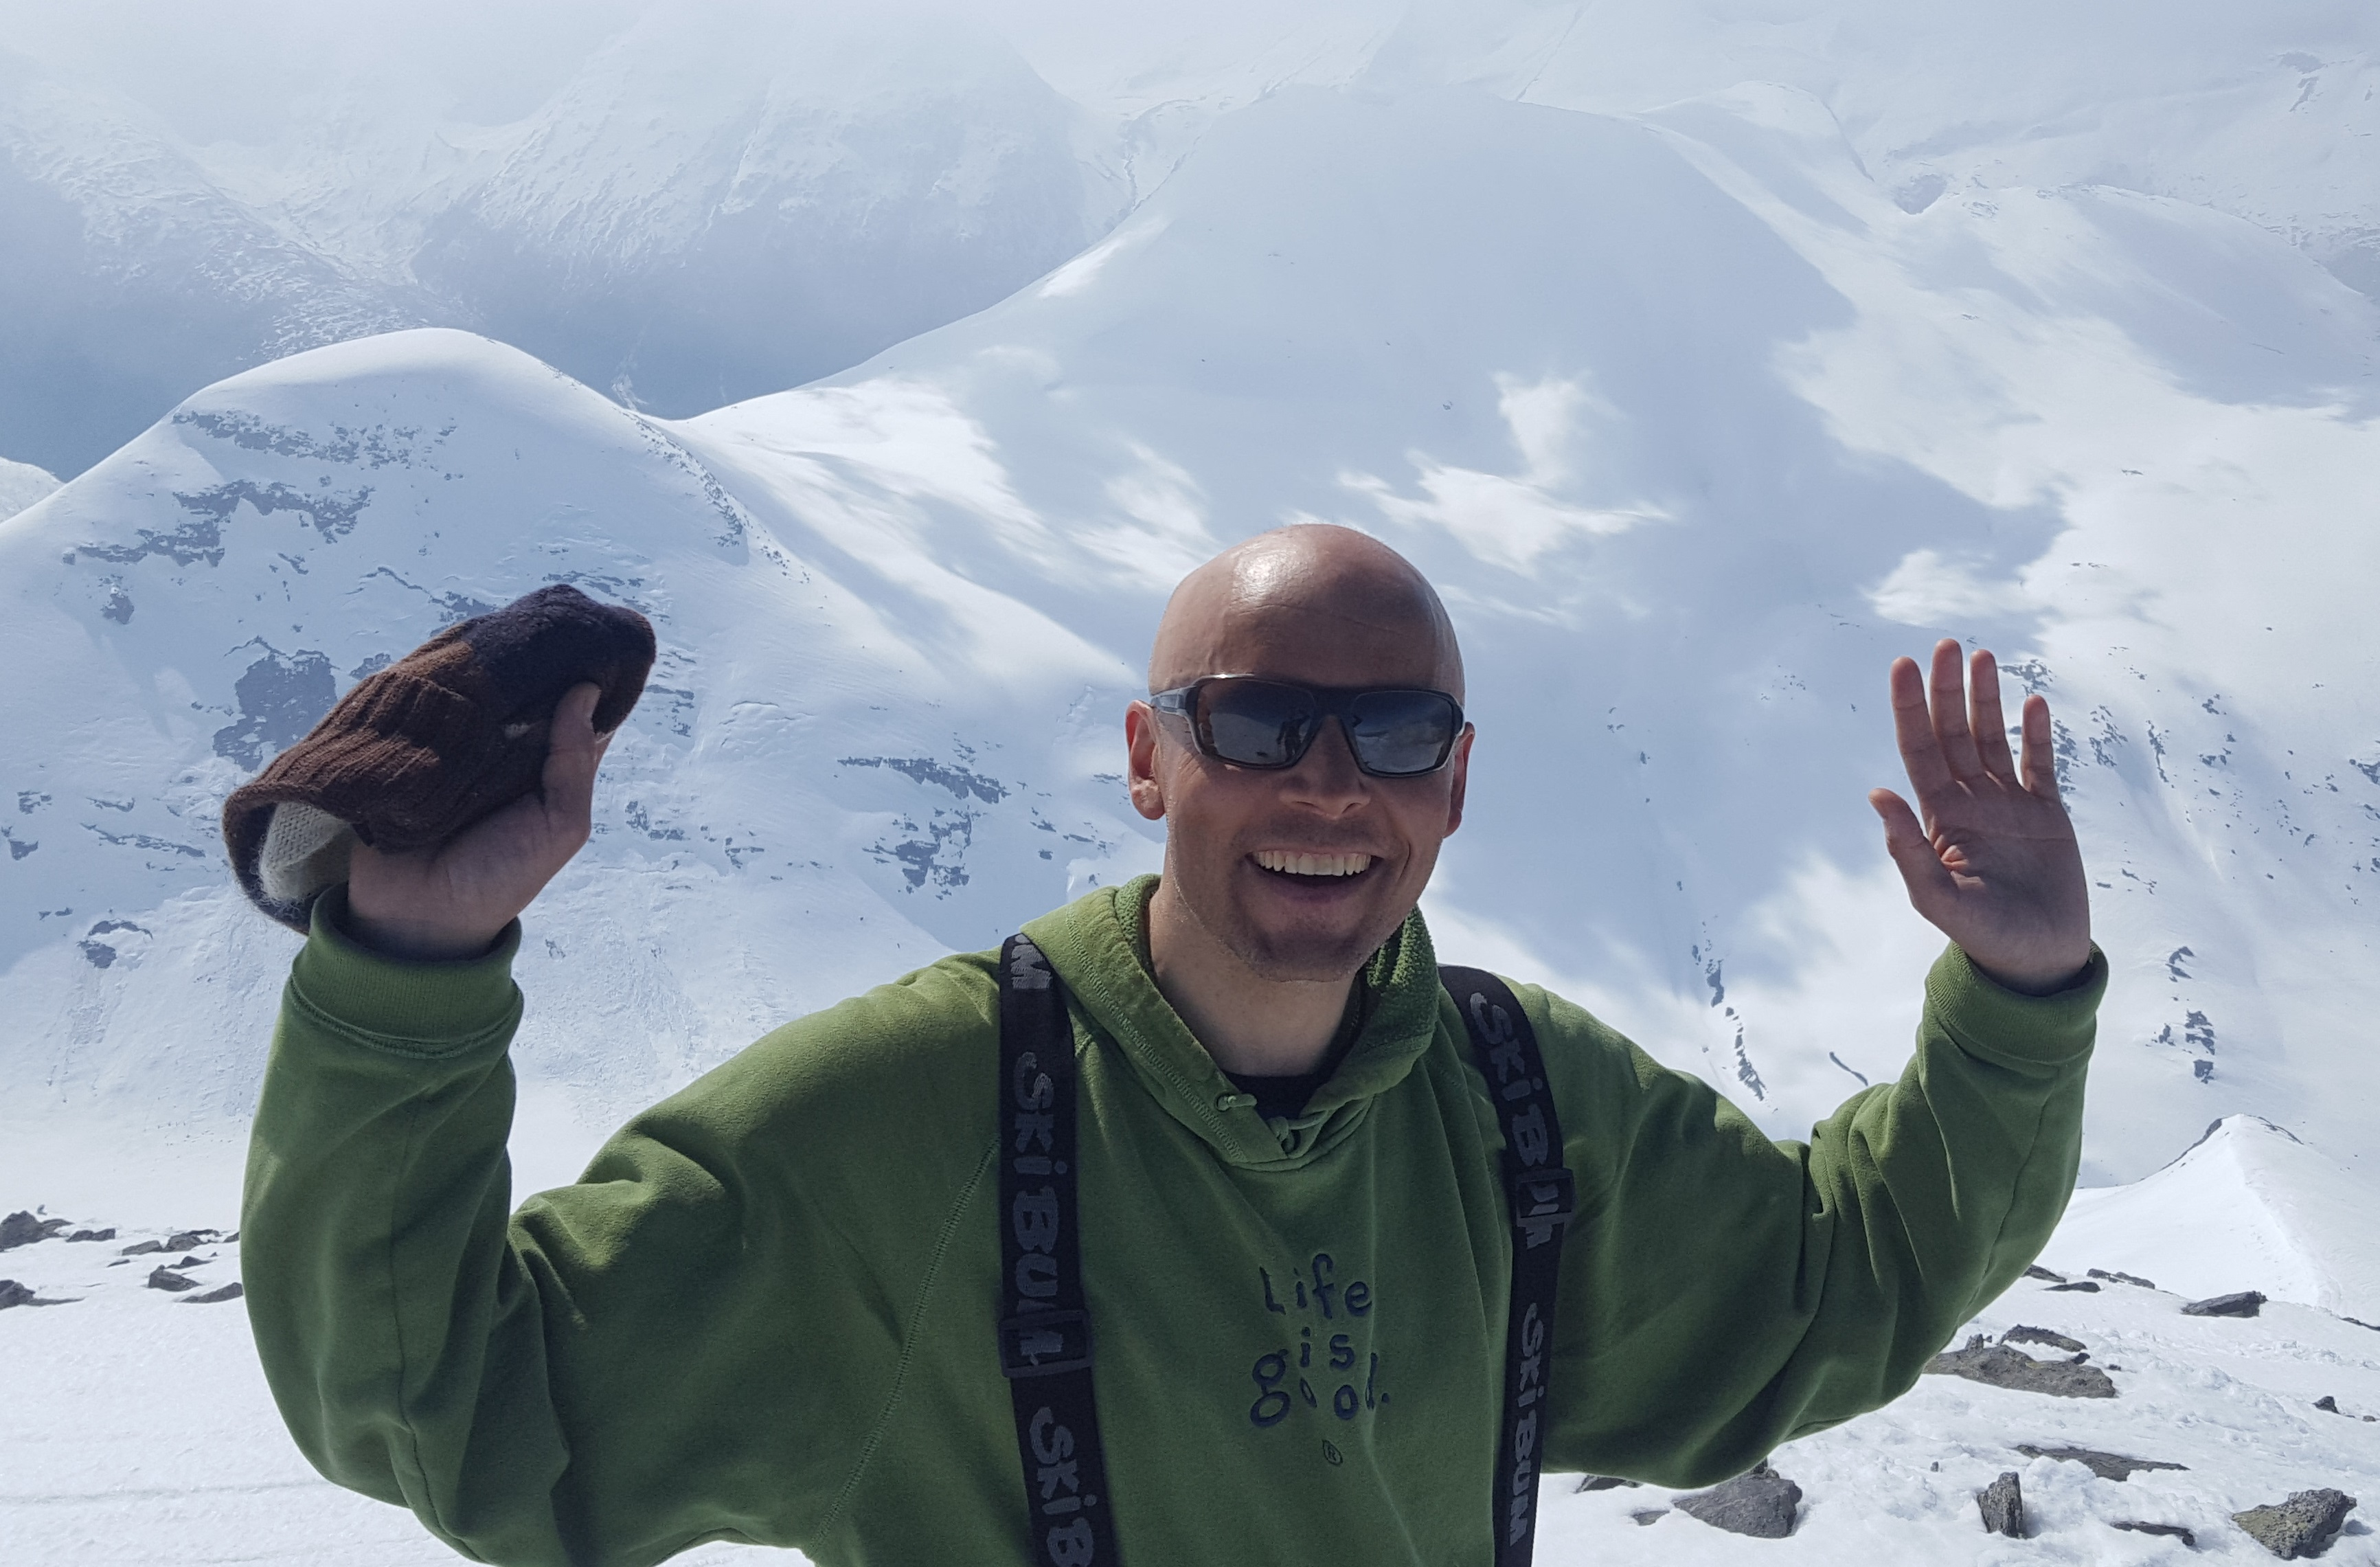
\includegraphics[scale=0.055]{fig/Eidsvikpicture.jpg}
\end{wrapfigure}
\textbf{Jo Eidsvik} is a Professor of Statistics at NTNU, Norway. His research profile is in spatial and computational statistics applied to the Earth sciences. He co-authored the book on Value of Information in the Earth Sciences (Cambridge Univ Press, 2015). He has industry experience from the Norwegian Research Defense Establishment and from Equinor. He is currently involved in several research projects on spatial and spatio-temporal modeling and monitoring, including ongoing work on autonomous maritime sampling and a center for geophysical forecasting.\\

\textbf{email: }\emph{jo.eidsvik@ntnu.no}\\
\textbf{Web: }\url{https://www.ntnu.no/employees/jo.eidsvik}
}

\vspace{20mm}

\parbox{6.5in}{
\begin{wrapfigure}{r}{3.6in - .75\columnsep} %{3.8in}{0.45\textwidth}
  % \centering
    \vspace{-\intextsep}
    \hspace*{-.35\columnsep}\includegraphics[scale=0.055]{fig/aida_snow_s.png}
\end{wrapfigure}
\textbf{Aida Alvera-Azcárate} is a researcher at the GeoHydrodynamics and Environment Research (GHER) group of the University of Liège (Belgium). She is a physical oceanographer specialised in the development of data analysis techniques for ocean remote sensing, like the gap-filling technique DINEOF (DataInterpolating Empirical Orthogonal Functions), widely used by oceanographers. She also enjoys studying the ocean dynamics from remote sensing data and the influence of ocean dynamics on the ecosystem. She is Associate Editor of Remote Sensing of Environment.\\

\textbf{email: }\emph{a.alvera@uliege.be}\\
\textbf{Web: }\url{http://labos.ulg.ac.be/gher/aida}
}
